\chapter{Requisitos do Sistema}

Os requisitos são capacidades que devem ser atendidas ou possuídas por um sistema para resolver um problema ou atingir um objetivo. O conjunto de todos os requisitos que formam a base para o desenvolvimento subsequente de um software \cite{vazquez2016}. Neles são definidos como serão os comportamentos do sistema e seus fluxos. Eles foram  abordados em dois segmentos: os requisitos funcionais que são fluxos do sistema e os requisitos não funcionais que são necessários para a utilização do sistema.

\section{Requisitos Funcionais}

Conforme \cite{sommerville2011software}, os requisitos funcionais de um sistema descrevem o que ele deve fazer, são dependentes do tipo de software a ser desenvolvido, de quem são seus possíveis usuários e da abordagem geral adotada pela organização ao escrever os requisitos. \cite{essi2005} define requisitos funcionais como necessidades descritas pelo cliente, onde a equipe do projeto analisa e especifica as funções, desempenho, interfaces e restrições, conforme as fases das metodologias aplicadas. Sua finalidade é distinguir as dependências do sistema para que o mesmo funcione de acordo com os requisitos informados pelo cliente.
\cite{sommerville2011software} acrescenta que quando os requisitos funcionais são expressos como requisitos de usuário, eles são normalmente descritos de forma abstrata, para serem compreendidos pelos usuários de sistema, entretanto, requisitos de sistema funcionais mais específicos descrevem em detalhes as funções do sistema como suas entradas e saídas.

A tabela \ref{tabela-requsitos-funcionais} demonstra os requisitos funcionais do sistema Agil.It, nela foi feito a separação por tipo de registro, que é disposto de cadastro, consulta e funcionalidade e o requisito em si.

\begin{table}[H]
	\centering
	\caption{\label{tabela-requsitos-funcionais}Requisitos Funcionais do Sistema Agil.It}
	\begin{tabular}{l|l}
		\hline
		\textbf{Tipo do Requisito} & \textbf{Requisito}                              \\ \hline
		Cadastro                   & Usuários                                       \\ \hline
		Cadastro                   & Centros de Trabalho                            \\ \hline
		Cadastro                   & Setores                                        \\ \hline
		Cadastro                   & Locais de Instalação                           \\ \hline
		Cadastro                   & Parametrizações de Segurança                   \\ \hline
		Cadastro                   & Tipos de Máquina                               \\ \hline
		Cadastro                   & Unidades de Medida                             \\ \hline
		Cadastro                   & Peças                                          \\ \hline
		Cadastro                   & Equipamentos                                   \\ \hline
		Cadastro                   & Equipamentos Superior                          \\ \hline
		Cadastro                   & Layouts de Ordem de Manutenção                 \\ \hline
		Cadastro                   & Causas do Defeito                              \\ \hline
		Cadastro                   & Sintomas do Defeito                            \\ \hline
		Cadastro                   & Observações Padrão                             \\ \hline
		Cadastro                   & Operações Padrão                               \\ \hline
		Cadastro                   & Ordens de Manutenção                           \\ \hline
		Consulta                   & Máquinas                                       \\ \hline
		Consulta                   & Ordens de Manutenção                           \\ \hline
		Funcionalidade             & Login                                          \\ \hline
		Funcionalidade             & Logoff                                         \\ \hline
		Funcionalidade             & Monitor de Ordens de Manutenção em Aberto      \\ \hline
		Funcionalidade             & Solicitação de Abertura de Ordem de Manutenção \\ \hline
		Funcionalidade             & Central de Notificação                         \\ \hline
	\end{tabular}
	\legend{Fonte: os autores (2020)}
\end{table}

\section{Requisitos Não Funcionais}

Requisitos não funcionais não estão diretamente ligados com os serviços específicos oferecidos pelo sistema a seus usuários. Eles podem estar relacionados às propriedades emergentes do sistema, como confiabilidade, tempo de resposta e ocupação de área \cite{sommerville2011software}. O propósito dos requisitos não funcionais é descrever as qualidades requeridas para um sistema, como sua usabilidade e seu desempenho \cite{IIBA2005}. Em sistemas alguns destes requisitos podem determinar tecnologias ou algoritmos específicos a serem utilizados, garantindo compatibilidade com sistemas existentes \cite{cordeiro2007}.

A tabela \ref{tabela-requsitos-nao-funcionais} demonstra os requisitos não funcionais do sistema Agil.It que foram definidos em conjunto com a empresa Duas Rodas.

\begin{table}[H]
	\centering
	\caption{\label{tabela-requsitos-nao-funcionais}Requisitos Não Funcionais do Sistema Agil.It}
	\begin{tabular}{l}
		\hline
		\multicolumn{1}{l}{\textbf{Requisto}}                                                 \\ \hline
		\multicolumn{1}{l}{Sistema Desenvolvido para Web}                                     \\ \hline
		\multicolumn{1}{l}{Versão Mobile para os Técnicos}                                    \\ \hline
		\multicolumn{1}{l}{Utilizar o Banco de Dados MS Sql Server}                           \\ \hline
		\multicolumn{1}{l}{Usuários Devem ter Acesso à Computadores e/ou Dispositivos Móveis} \\ \hline
	\end{tabular}
	\legend{Fonte: os autores (2020)}
\end{table}

\section{Fluxograma do Sistema Desenvolvido}

Segundo \cite{pejeronimo2002} fluxograma é uma representação gráfica das tarefas de um determinado processo, sendo de forma sequencial a execução delas. \cite{roberthurt} relata que um fluxograma fornece um panorama de alto nível sobre um sistema de informação.

As formas geométricas têm a finalidade de direcionar o fluxo da informação ao usuário enquanto as linhas e setas descrevem a sequência das atividades, mostrando o caminho da informação de modo estruturado e as transformações à medida que os dados vão se movimentando desde a entrada até a saída \cite{souza2017desenvolvimento}.

\begin{figure}[H]
	\caption{\label{flux_sys}Fluxo do AGIL.IT}
	\begin{center}
		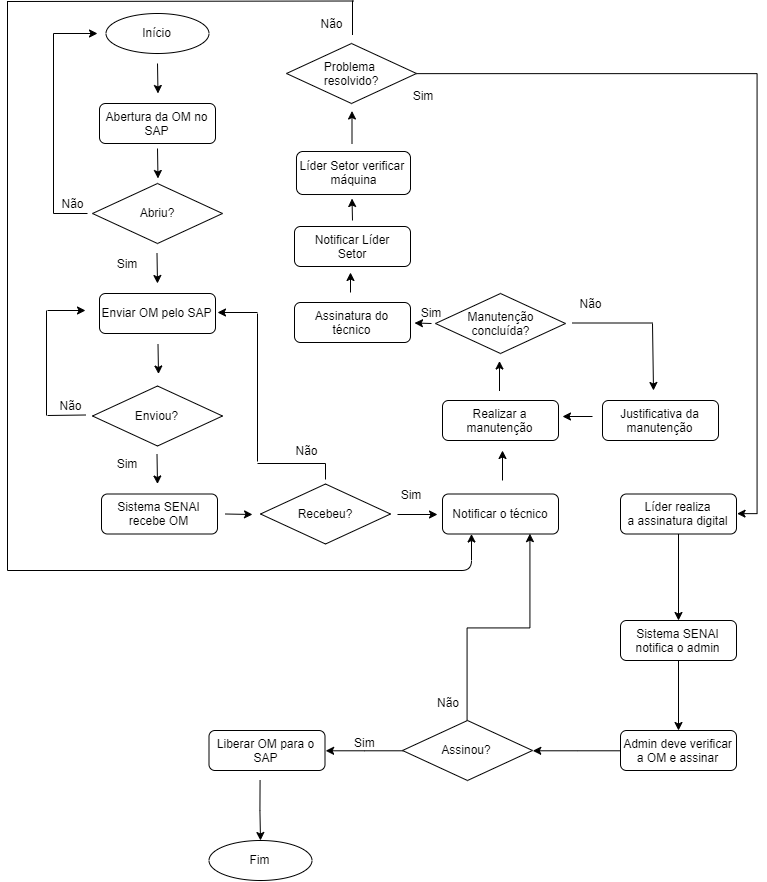
\includegraphics[scale=0.55]{./Figuras/fluxo-sistema.png}
	\end{center}
	\legend{Fonte: os autores (2020)}
\end{figure}

Na Figura \ref{flux_sys} é possível verificar todo o fluxo do sistema onde começa e termina com a integração do SAP.
O sistema irá receber a OM do SAP e notificar o técnico responsável pela execução do serviço. Após o técnico realizar a manutenção, os usuários (técnico, e líder do setor) realizam as assinaturas e o usuário administrador analisa e libera a OM para a integração.

	
\section{Diagrama de Caso de Uso do Sistema}

Diagramas dos casos de uso são técnicas utilizadas para captar os requisitos funcionais de um sistema, descrevem as interações entre usuários de um sistema e o próprio sistema, fornecendo uma narrativa sobre como ele é utilizado \cite{umlessencial2005}.
	
Para \cite{carniello2003} seu objetivo principal consiste em definir o comportamento de um sistema, sem revelar sua estrutura interna.

Em sua forma mais simples, um caso de uso identifica os atores envolvidos em uma interação e dá nome ao tipo de interação, ela pode ser complementada por informações adicionais que descrevem a interação com o sistema. Essas informações adicionais podem ser descritas textualmente ou por modelos gráficos \cite{sommerville2011software}.

\begin{figure}[htb]
	\caption{\label{caso_uso}Caso de Uso do AGIL.IT}
	\begin{center}
		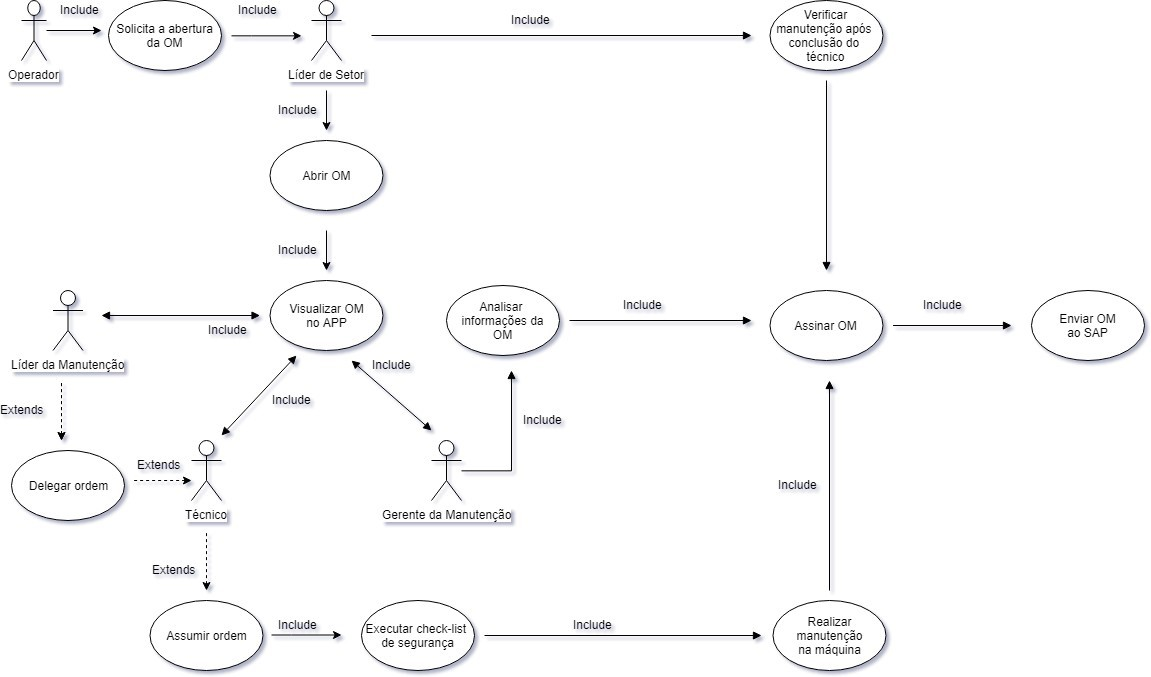
\includegraphics[scale=0.57]{./Figuras/caso-uso.png}
	\end{center}
	\legend{Fonte: os autores (2020)}
\end{figure}

Na Figura \ref{caso_uso} é possível verificar quais ações cada ator desempenhará no sistema. Os operadores de máquinas e os líderes de manutenção verificam a manutenção feita e assinam a OM. O técnico realizará a manutenção e verificará as peças necessárias para realizar a assistência ao equipamento e se as mesmas possuem estoque disponível. E o administrador realizará cadastros e encerrará as ordens de manutenção.

	
\section{Modelo Entidade-Relacionamento do Banco de Dados}

Utilizar o modelo entidade-relacionamento, tem como objetivo, obter uma descrição de forma abstrata dos dados que serão armazenados no banco de dados \cite{2010_erbd}.

Como o próprio nome sugere, o modelo entidade-relacionamento é composto por entidades e relacionamentos. Entidades possuem um nome e um ou mais atributos que podem ser compostos ou simples, enquanto os relacionamentos são utilizados para montar a ligação entre as entidades \cite{noguera2018extensao}. A entidade pode ser forte, se não depender de outra para existir ou fraca, se sua existência no modelo estiver condicionada à presença de outra entidade \cite{dantas2016analise}.

\begin{figure}[H]
	\caption{\label{entidade_relacionamento}Entidade de Relacionamento}
	\begin{center}
		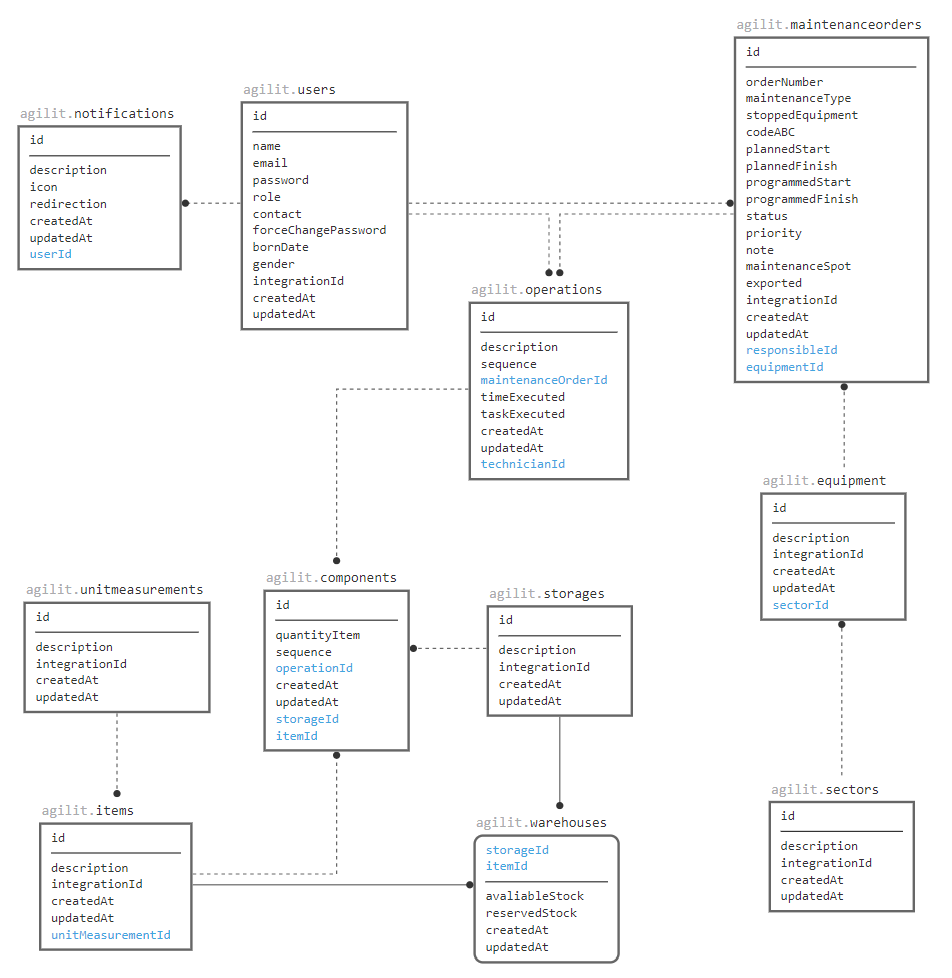
\includegraphics[scale=0.70]{./Figuras/er3.png}
	\end{center}
	\legend{Fonte: os autores (2020)}
\end{figure}

A Figura \ref{entidade_relacionamento} mostra toda a entidade de relacionamento do banco de dados, onde cada tabela representa uma estrutura de dados no banco de dados e as ligações entre elas demonstram relacionamentos que essas tabelas possuem entre si.

%------------------------------------------------------------------------